\newgeometry{
    a4paper,
    top=24mm,
    bottom=28mm,
    left=39mm,
    right=39mm,
    heightrounded
}
\partpage{Esercitazioni}
\restoregeometry

\chapter{Datazione}

Una delle applicazioni più note della radioattività è la datazione, cioè la misura dell'età di un campione a partire dalla sua composizione isotopica. 

L'idea di fondo è sempre la stessa: un nucleo radioattivo decade con una costante $\lambda$ fissata, che non dipende dalle condizioni esterne come temperatura o pressione. Il rapporto tra il numero di nuclei padre e il numero di nuclei figli accumulati funziona quindi da \emph{orologio}, purché si conosca la composizione del campione all'istante iniziale e purché il sistema sia rimasto chiuso, cioè non ci siano stati scambi con l'ambiente. 

La scelta dell'isotopo dipende dalla scala di tempi che si vuole misurare: l'orologio è utile finché non è passato troppo tempo rispetto alla vita media, altrimenti il nucleo padre è ormai scomparso. Per le rocce si usano quindi nuclei con vite medie dell'ordine del miliardo di anni, come gli isotopi dell'uranio, mentre per i reperti archeologici si ricorre al $^{14}\mathrm{C}$, che ha una vita media di qualche migliaio di anni.\\

\section{Datazione con U - Pb}

Andiamo a sfruttare quanto studiato sul decadimento dei nuclei per ottenere una datazione delle rocce in cui si ha una catena di decadimento $U - Pb$.

Gli isotopi dell'uranio $^{235}U$ e $^{238}U$ fanno una serie di decadimenti fino ad arrivare, rispettivamente, a $^{207}Pb$ e $^{206}Pb$, che sono atomi stabili. 
%
\begin{align}
    ^{235}U \longrightarrow  \cdots \longrightarrow \ ^{207}&Pb \qquad T_{1/2}^{235} = 7 \cdot 10^{8} \ y\\
    ^{238}U \longrightarrow  \cdots \longrightarrow \ ^{206}&Pb \qquad T_{1/2}^{238} = 4,5 \cdot 10^{9} \ y
\end{align}
L'orologio consiste nel misurare il rapporto $N_{Pb}(t)/N_{U}(t)$, dove $t = 0$ corrisponte al momento in cui l'uranio è stato creato (che corrisponde alla ``nascita'' della roccia), mentre $t$ corrisponde ad adesso.\\
Sappiamo che il numero di atomi di uranio in funzione del tempo corrisponde a 
%
\begin{equation*}
    N_{U}(t) = N_0 e^{-\lambda_U t}
\end{equation*}
Inoltre, se supponiamo che all'istante iniziale il numero di atomi di piombo sia \emph{nullo} e che il sistema sia chiuso si ha che 
%
\begin{equation}
    N_{Pb}(t) = N_0 - N_{U}(t) = N_0 (1 - e^{- \lambda_U t})
    \label{eq:numero_Pb}
\end{equation}
Quindi il rapporto tra queste due quantità risulta essere 
% 
\begin{tcolorbox}[colback=yellow!10!white, colframe=orange!70!black, boxrule=0.8pt]
\begin{equation}
    \frac{N_{Pb}(t)}{N_{U}(t)}  = e^{\lambda_U t} - 1
\end{equation}
\end{tcolorbox}
Questo risultato mi permette di ottenere la datazione di una roccia a partire dal rapporto tra $U$ e $Pb$ che trovo \emph{ora} nella roccia.\\

Dato che abbiamo due catene di decadimenti in base all'isotopo di uranio iniziale, possiamo andare a considerare due orologi. \\
Tornando alla relazione precedente, possiamo scrivere un orologio per ciascuna delle due catene e definire le due quantità
%
\begin{align}
    x & \equiv \frac{N_{Pb207}(t)}{N_{U235}(t)} = e^{\lambda_{235} t} - 1 \\
    y & \equiv \frac{N_{Pb206}(t)}{N_{U238}(t)} = e^{\lambda_{238} t} - 1
\end{align}
Se le ipotesi fatte sono corrette (sistema chiuso e assenza di piombo iniziale) i due orologi devono segnare tempi compatibili, cioè lo stesso $t$. 

Possiamo allora ricavare il tempo dal primo orologio
%
\begin{equation*}
    t = \frac{\ln(1 + x)}{\lambda_{235}}
\end{equation*}
e sostituirlo nel secondo, ottenendo una relazione che lega direttamente $x$ e $y$
%
\begin{equation*}
    y = \exp \left[ \frac{\lambda_{238}}{\lambda_{235}} \ln(1+x) \right] - 1
\end{equation*}
cioè
%
\begin{tcolorbox}[colback=yellow!10!white, colframe=orange!70!black, boxrule=0.8pt]
\begin{equation}
    y = (1 + x)^{\frac{\lambda_{238}}{\lambda_{235}}} - 1
\end{equation}
\end{tcolorbox}
Questa curva, introdotta da Wetherill, prende il nome di curva della concordia\mkeyword{curva della concordia}. 

\begin{figure}[htbp]
\centering
\begin{tikzpicture}[x=0.16cm, y=6cm]

% assi
\draw[->] (0,0) -- (58,0) node[anchor=north east] {$x$};
\draw[->] (0,0) -- (0,1.1) node[anchor=south east] {$y$};

% curva della concordia
\draw[thick, domain=0:52, samples=200, smooth] plot (\x, {pow(1+\x,0.158)-1});
\node[rotate=13] at (32,0.78) {concordia};

% retta della discordia
\draw[thick, dashed] (0,0.158) -- (50,0.960);
\node[rotate=9] at (26,0.44) {discordia};

% intersezioni
\fill (2,0.190) circle (1.5pt);
\fill (40,0.800) circle (1.5pt);

\end{tikzpicture}
\caption{Diagramma di Wetherill.}
\label{fig:concordia}
\end{figure}
Poiché $\lambda_{238} < \lambda_{235}$ l'esponente è minore di $1$ e la curva risulta crescente e concava: ogni suo punto corrisponde a una roccia di una certa età, che si legge scorrendo la curva. 

Non sempre però i dati sperimentali giacciono sulla concordia. In questo caso i punti si dispongono lungo una retta detta discordia\mkeyword{discordia}, segno che il sistema non è rimasto chiuso, ad esempio per una perdita di piombo successiva alla formazione della roccia. 

\subsection{Precisazione sul decadimento}

Prima di continuare è necessario fare una precisazione sulla relazione \eqref{eq:numero_Pb} usata nella sezione precedente. 

La catena di decadimento che porta dall'uranio al piombo non è diretta, ma passa attraverso una serie di nuclei intermedi 
%
\begin{equation*}
    {}^{238}\mathrm{U} \longrightarrow \mathrm{Th} \longrightarrow \mathrm{Pa} \longrightarrow \mathrm{U} \longrightarrow \cdots \longrightarrow {}^{206}\mathrm{Pb}
\end{equation*}
Di conseguenza la relazione $N_{Pb} = N_0 - N_U$ non è esatta, perché una parte dei nuclei iniziali si trova in uno degli stadi intermedi. Il bilancio corretto è infatti
%
\begin{equation*}
    N_0 = N_{U}(t) + \sum_i N_i(t) + N_{Pb}(t)
\end{equation*}
dove la somma è estesa a tutti i nuclei intermedi della catena, da cui
%
\begin{equation}
    N_{Pb}(t) = N_0 - N_{U}(t) - \sum_i N_i(t)
    \label{eq:bilancio_esatto}
\end{equation}
Per recuperare la relazione usata sopra sfruttiamo l'equilibrio secolare. Il capostipite ha infatti una vita media enormemente più lunga di quella di tutti i suoi discendenti
%
\begin{equation*}
    T_{1/2}({}^{238}\mathrm{U}) \gg T_{1/2}(i) \qquad \forall i
\end{equation*}
e quindi la catena si trova in equilibrio secolare, per cui tutte le attività sono uguali
%
\begin{equation*}
    \lambda_i N_i = \lambda_{238} N_{238} \qquad \Longrightarrow \qquad N_i = \frac{\lambda_{238}}{\lambda_i} N_{238}
\end{equation*}
Poiché $\lambda_i \gg \lambda_{238}$, il rapporto $\lambda_{238}/\lambda_i$ è trascurabile e con esso lo è il numero di nuclei intermedi presenti a ogni istante. La \eqref{eq:bilancio_esatto} diventa quindi 
%
\begin{tcolorbox}[colback=yellow!10!white, colframe=orange!70!black, boxrule=0.8pt]
\begin{equation}
    N_{Pb}(t) = N_0 - N_{U}(t) - \sum_i N_i(t) \simeq N_0 - N_U(t)
\end{equation}
\end{tcolorbox}
In altre parole, i nuclei intermedi funzionano da semplice canale di transito: appena si formano decadono, e in ogni istante ce n'è una quantità trascurabile rispetto a $N_0$.

\newpage

\section{Datazione con $^{14}C$}

Il metodo del $^{14}C$, o metodo del radiocarbonio, è un metodo di datazione di materiale organico basato sulla misura delle abbondanze relative del $^{14}C$, un isotopo radioattivo del carbonio.\\
Il decadimento di questo isotopo di carbonio è 
%
\begin{equation}
    ^{14}C \to \ ^{14}N + e^- + \bar{\nu}
\end{equation}

Il carbonio-14 è presente nell'atmosfera perché viene continuamente prodotto dai raggi cosmici, che interagendo con i nuclei dell'aria generano neutroni; questi, catturati dall'azoto, danno luogo alla reazione
%
\begin{equation*}
    {}^{14}\mathrm{N} + n \longrightarrow {}^{14}\mathrm{C} + p
\end{equation*}
Dall'atmosfera, poi, passa alla biosfera. 

Finché l'organismo è vivo continua a scambiare carbonio con l'ambiente, attraverso la respirazione e l'alimentazione, e mantiene quindi un rapporto isotopico pari a quello atmosferico. Consideriamo allora il rapporto
%
\begin{equation}
    R_0 = \left. \frac{{}^{14}\mathrm{C}}{{}^{12}\mathrm{C}} \right|_{\text{atm}}
\end{equation}
che è il valore presente nell'atmosfera, e quindi nell'organismo, subito prima della morte. 

Alla morte lo scambio si interrompe: il $^{12}\mathrm{C}$ resta costante, mentre il $^{14}\mathrm{C}$ decade senza più essere rimpiazzato. Il rapporto misurato oggi vale quindi
%
\begin{equation}
    R(t) = \frac{N_{14}(t)}{N_{12}(t)} = \frac{N_{14}(0) e^{-\lambda_{14} t}}{N_{12}(0)} = R_0 \, e^{-\lambda_{14} t}
\end{equation}
dove $t = 0$ è il momento in cui l'organismo che vogliamo datare è morto. Invertendo si ottiene l'età del reperto
%
\begin{tcolorbox}[colback=yellow!10!white, colframe=orange!70!black, boxrule=0.8pt]
\begin{equation}
    t = \frac{1}{\lambda_{14}} \ln \left( \frac{R_0}{R(t)} \right)
\end{equation}
\end{tcolorbox}

\subsection{Calibrazione}

Il problema di questo metodo è che $R_0$ \emph{non è costante nel tempo}: la produzione di $^{14}\mathrm{C}$ dipende dal flusso di raggi cosmici, che varia con l'attività solare e con il campo magnetico terrestre. Per usare la tecnica serve quindi una calibrazione. 

Un modo è considerare gli anelli degli alberi: ogni anello corrisponde a un anno noto con certezza e conserva il carbonio fissato in quell'anno, per cui misurandone il $^{14}\mathrm{C}$ si ricostruisce $R_0$ anno per anno\footnote{Questa tecnica prende il nome di dendrocronologia e permette di risalire indietro di diverse migliaia di anni; per epoche più remote si usano altri archivi, come i coralli o le stalagmiti.}. 

Si costruisce così una curva di calibrazione che lega l'età ricavata dal decadimento (\emph{radiocarbon age}) all'anno di calendario. Se $R_0$ fosse davvero costante la curva sarebbe una retta, mentre quella reale oscilla attorno a questo andamento ideale. 

\begin{figure}[h]
  \centering
  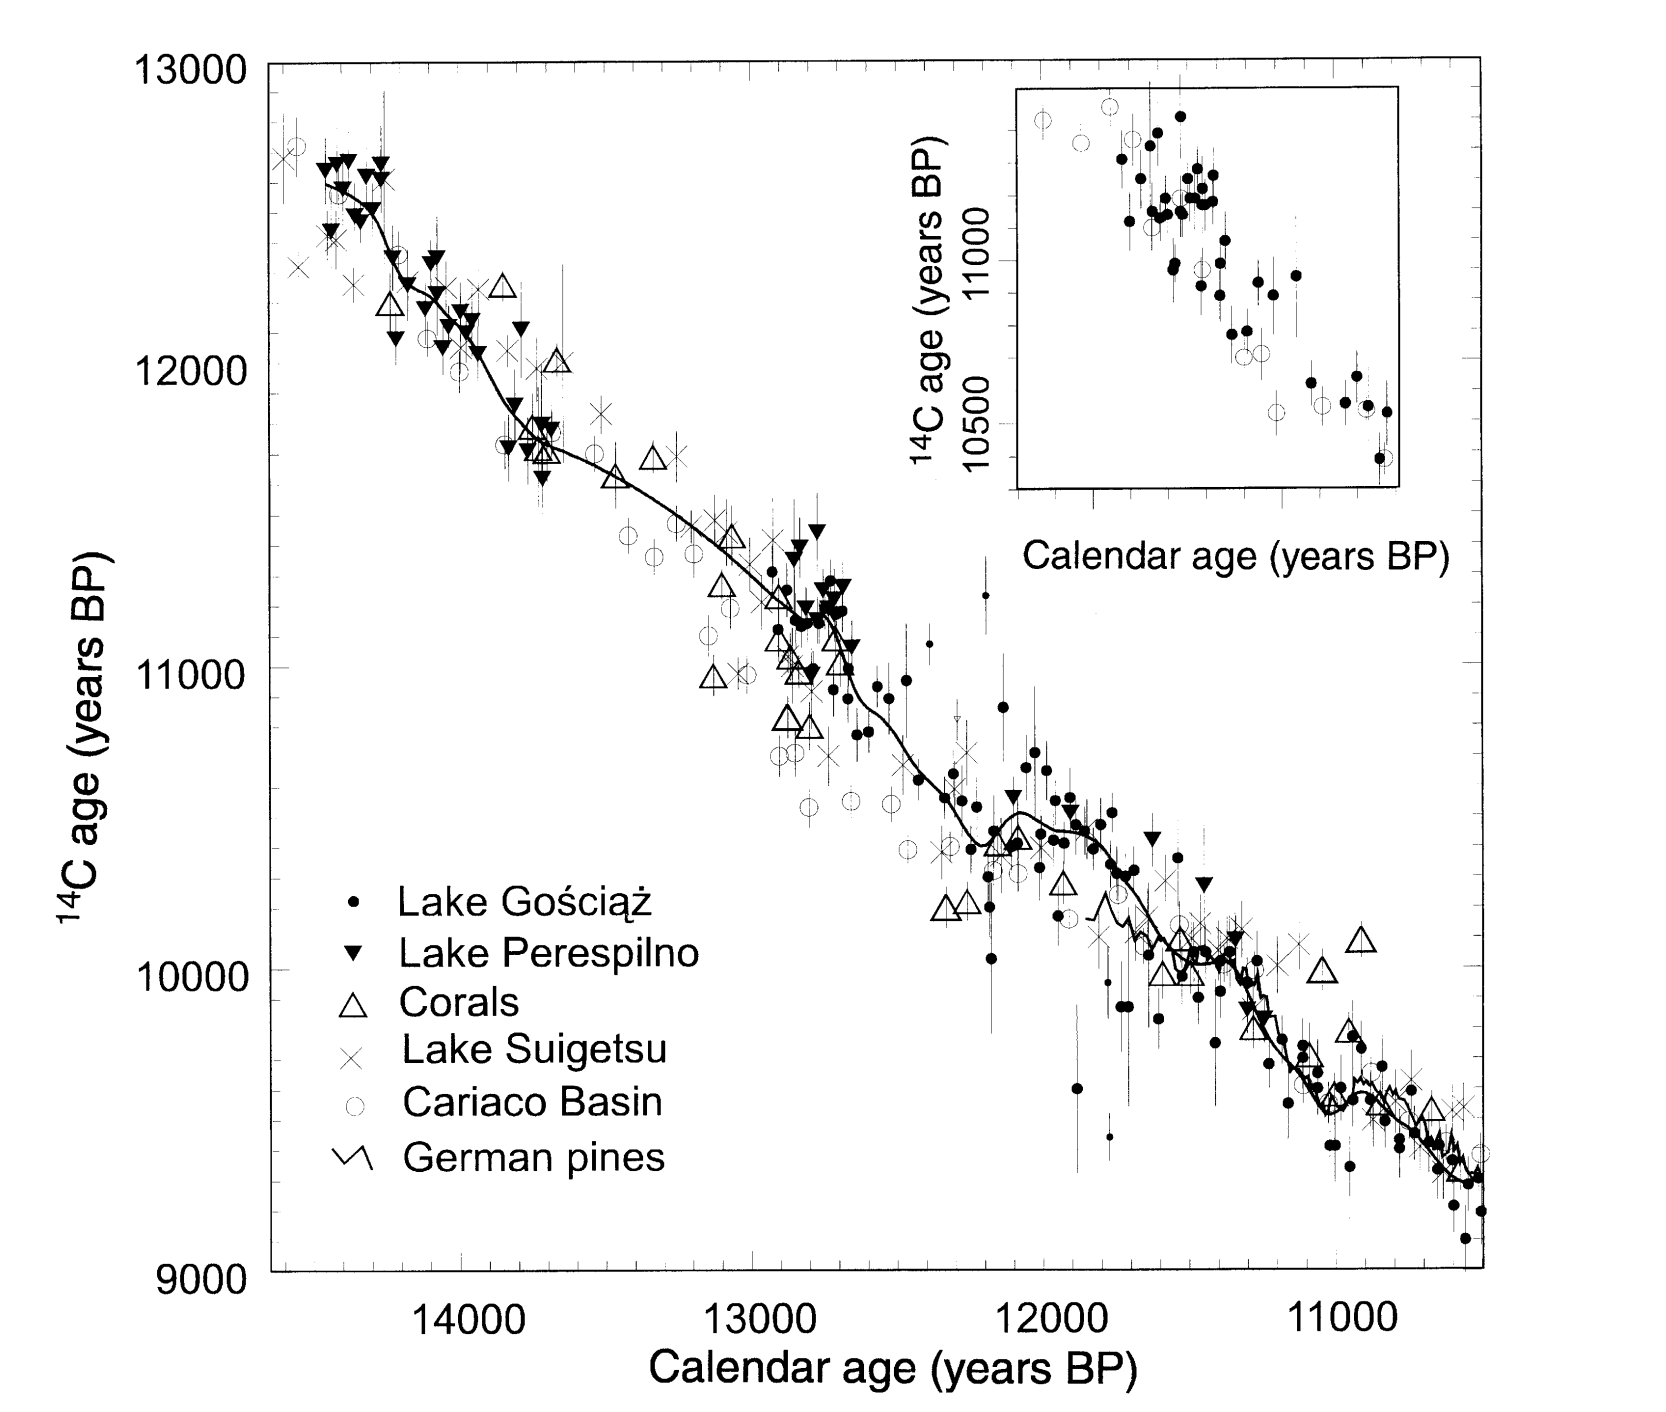
\includegraphics[width=0.75\linewidth]{foto/Radiocarbonage.png}
  \caption{Curva di calibrazione del radiocarbonio}
  \label{fig:etichetta}
\end{figure}

% \begin{figure}[htbp]
% \centering
% \begin{tikzpicture}[x=0.11cm, y=0.055cm]

% % assi
% \draw[->] (0,0) -- (0,105) node[anchor=south west, align=left] {radiocarbon\\ age};
% \draw[->] (0,0) -- (110,0) node[anchor=north west, align=left] {calendar\\ year};

% % curva ideale
% \draw[gray] (10,95) -- (100,8);
% \node[gray, anchor=north west] at (72,28) {ideale};

% % curva reale
% \draw[thick, smooth] plot coordinates {
%     (10,95) (16,72) (22,78) (28,74) (34,58) (40,52) (46,56) (52,48)
%     (58,25) (61,24) (64,58) (67,57) (70,30) (76,32) (82,20) (88,18) (94,10) (100,8)
% };
% \node[anchor=west] at (66,64) {reale};

% % lettura di una data
% \draw[dashed, gray] (0,95) -- (10,95);
% \draw[dashed, gray] (10,95) -- (10,0);
% \node[anchor=east] at (0,95) {$t$};

% \end{tikzpicture}
% \caption{Curva di calibrazione del radiocarbonio.}
% \label{fig:calibrazione}
% \end{figure}

Il fatto che la curva reale non sia monotòna è un limite intrinseco del metodo: a una stessa età radiometrica possono corrispondere più anni di calendario, e la datazione non può quindi essere resa arbitrariamente precisa. 

Inoltre la curva va corretta tenendo conto degli effetti antropici che hanno alterato il rapporto isotopico atmosferico, come l'immissione di carbonio fossile, privo di $^{14}\mathrm{C}$, e i test nucleari atmosferici degli anni Cinquanta e Sessanta, che ne hanno invece raddoppiato la concentrazione.